\documentclass{standalone}
\usepackage{tikz}
\usetikzlibrary{patterns, positioning}

\begin{document}
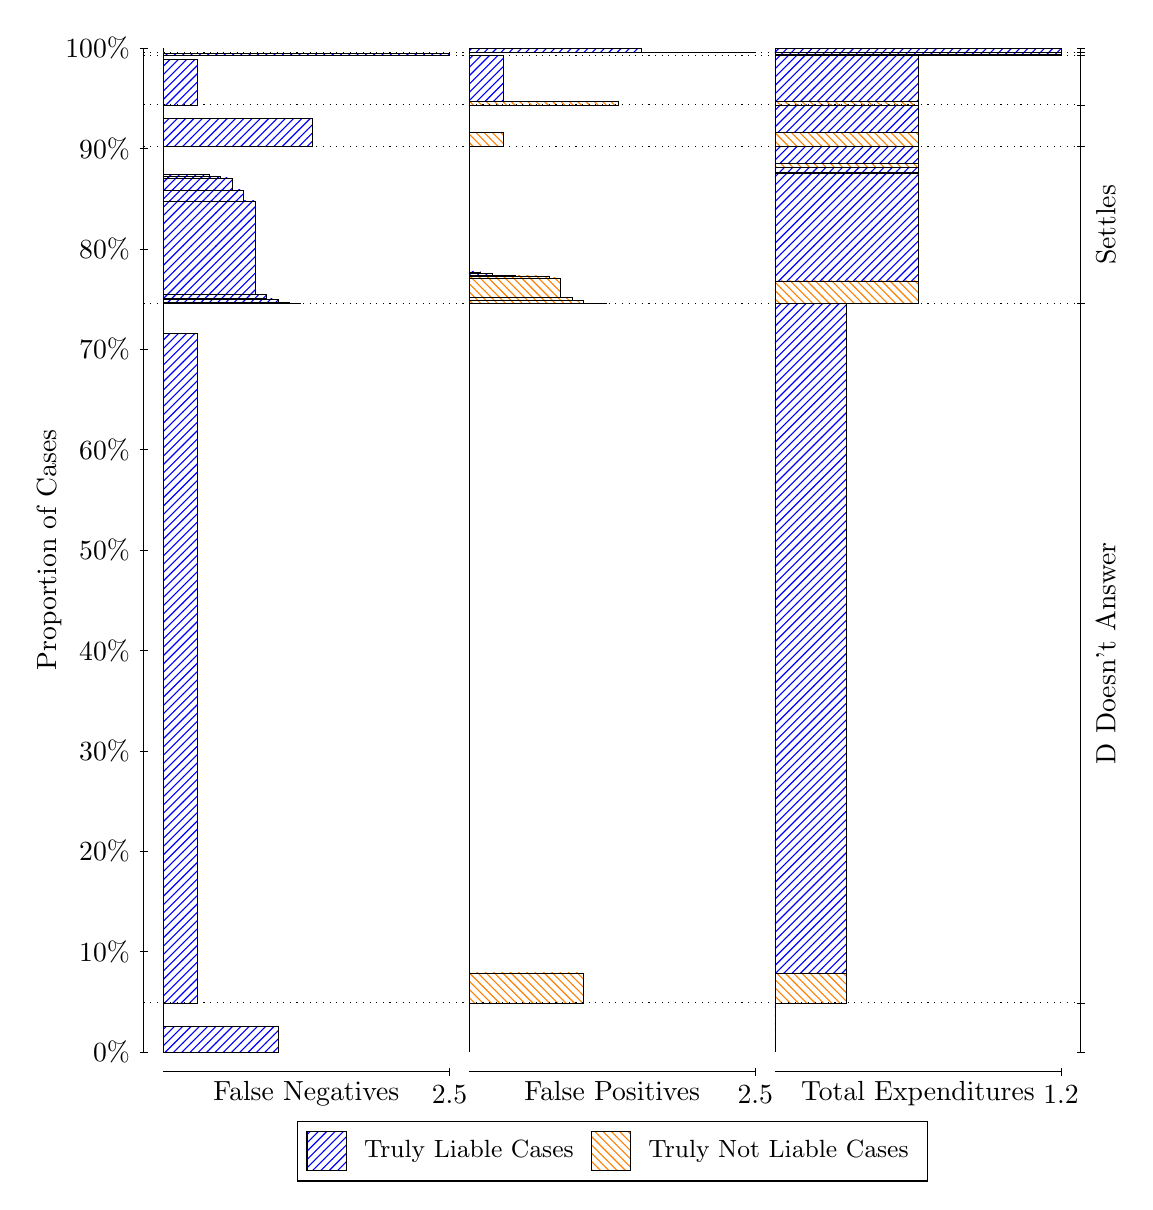
\begin{tikzpicture}
\draw[black, very thin] (1.5,1.75) -- (1.5,14.5);
\node[rotate=90, anchor=center] at (0.3, 8.125) {Proportion of Cases};
\draw[black, very thin] (1.45,1.75) -- (1.55,1.75);
\node[anchor=east] at (1.45, 1.75) {0\%};
\draw[black, very thin] (1.45,3.025) -- (1.55,3.025);
\node[anchor=east] at (1.45, 3.025) {10\%};
\draw[black, very thin] (1.45,4.3) -- (1.55,4.3);
\node[anchor=east] at (1.45, 4.3) {20\%};
\draw[black, very thin] (1.45,5.575) -- (1.55,5.575);
\node[anchor=east] at (1.45, 5.575) {30\%};
\draw[black, very thin] (1.45,6.85) -- (1.55,6.85);
\node[anchor=east] at (1.45, 6.85) {40\%};
\draw[black, very thin] (1.45,8.125) -- (1.55,8.125);
\node[anchor=east] at (1.45, 8.125) {50\%};
\draw[black, very thin] (1.45,9.4) -- (1.55,9.4);
\node[anchor=east] at (1.45, 9.4) {60\%};
\draw[black, very thin] (1.45,10.675) -- (1.55,10.675);
\node[anchor=east] at (1.45, 10.675) {70\%};
\draw[black, very thin] (1.45,11.95) -- (1.55,11.95);
\node[anchor=east] at (1.45, 11.95) {80\%};
\draw[black, very thin] (1.45,13.225) -- (1.55,13.225);
\node[anchor=east] at (1.45, 13.225) {90\%};
\draw[black, very thin] (1.45,14.5) -- (1.55,14.5);
\node[anchor=east] at (1.45, 14.5) {100\%};

\draw[black, very thin] (13.4,1.75) -- (13.4,14.5);
\draw[black, very thin] (13.35,1.75) -- (13.45,1.75);
\node[anchor=west] at (13.35, 1.75) {};
\draw[black, very thin] (13.35,2.374) -- (13.45,2.374);
\node[anchor=west] at (13.35, 2.374) {};
\draw[black, very thin] (13.35,11.254) -- (13.45,11.254);
\node[anchor=west] at (13.35, 11.254) {};
\draw[black, very thin] (13.35,13.253) -- (13.45,13.253);
\node[anchor=west] at (13.35, 13.253) {};
\draw[black, very thin] (13.35,13.778) -- (13.45,13.778);
\node[anchor=west] at (13.35, 13.778) {};
\draw[black, very thin] (13.35,14.404) -- (13.45,14.404);
\node[anchor=west] at (13.35, 14.404) {};
\draw[black, very thin] (13.35,14.441) -- (13.45,14.441);
\node[anchor=west] at (13.35, 14.441) {};
\draw[black, very thin] (13.35,14.5) -- (13.45,14.5);
\node[anchor=west] at (13.35, 14.5) {};

\draw[black, very thin, pattern color=blue, pattern=north east lines] (1.75,1.75) rectangle (3.2033,2.0708);
\draw[black, very thin, pattern color=orange, pattern=north west lines] (1.75,2.0708) rectangle (1.75,2.374);
\draw[black, very thin, pattern color=blue, pattern=north east lines] (1.75,2.374) rectangle (2.186,10.873);
\draw[black, very thin, pattern color=orange, pattern=north west lines] (1.75,10.873) rectangle (1.75,11.254);
\draw[black, very thin, pattern color=blue, pattern=north east lines] (1.75,11.254) rectangle (3.494,11.261);
\draw[black, very thin, pattern color=blue, pattern=north east lines] (1.75,11.261) rectangle (3.3487,11.266);
\draw[black, very thin, pattern color=blue, pattern=north east lines] (1.75,11.266) rectangle (3.2033,11.314);
\draw[black, very thin, pattern color=blue, pattern=north east lines] (1.75,11.314) rectangle (3.058,11.319);
\draw[black, very thin, pattern color=blue, pattern=north east lines] (1.75,11.319) rectangle (3.058,11.369);
\draw[black, very thin, pattern color=blue, pattern=north east lines] (1.75,11.369) rectangle (2.9127,12.558);
\draw[black, very thin, pattern color=blue, pattern=north east lines] (1.75,12.558) rectangle (2.7673,12.697);
\draw[black, very thin, pattern color=blue, pattern=north east lines] (1.75,12.697) rectangle (2.622,12.85);
\draw[black, very thin, pattern color=blue, pattern=north east lines] (1.75,12.85) rectangle (2.4767,12.87);
\draw[black, very thin, pattern color=blue, pattern=north east lines] (1.75,12.87) rectangle (2.3313,12.898);
\draw[black, very thin, pattern color=orange, pattern=north west lines] (1.75,12.898) rectangle (1.75,13.253);
\draw[black, very thin, pattern color=blue, pattern=north east lines] (1.75,13.253) rectangle (3.6393,13.605);
\draw[black, very thin, pattern color=orange, pattern=north west lines] (1.75,13.605) rectangle (1.75,13.778);
\draw[black, very thin, pattern color=blue, pattern=north east lines] (1.75,13.778) rectangle (2.186,14.358);
\draw[black, very thin, pattern color=orange, pattern=north west lines] (1.75,14.358) rectangle (1.75,14.404);
\draw[black, very thin, pattern color=blue, pattern=north east lines] (1.75,14.404) rectangle (5.3833,14.428);
\draw[black, very thin, pattern color=orange, pattern=north west lines] (1.75,14.428) rectangle (1.75,14.441);
\draw[black, very thin, pattern color=orange, pattern=north west lines] (1.75,14.441) rectangle (1.75,14.443);
\draw[black, very thin, pattern color=blue, pattern=north east lines] (1.75,14.443) rectangle (1.75,14.5);
\draw[black, very thin, pattern color=orange, pattern=north west lines] (5.6333,1.75) rectangle (5.6333,2.0532);
\draw[black, very thin, pattern color=blue, pattern=north east lines] (5.6333,2.0532) rectangle (5.6333,2.374);
\draw[black, very thin, pattern color=orange, pattern=north west lines] (5.6333,2.374) rectangle (7.0867,2.7555);
\draw[black, very thin, pattern color=blue, pattern=north east lines] (5.6333,2.7555) rectangle (5.6333,11.254);
\draw[black, very thin, pattern color=orange, pattern=north west lines] (5.6333,11.254) rectangle (7.3773,11.256);
\draw[black, very thin, pattern color=orange, pattern=north west lines] (5.6333,11.256) rectangle (7.232,11.258);
\draw[black, very thin, pattern color=orange, pattern=north west lines] (5.6333,11.258) rectangle (7.0867,11.294);
\draw[black, very thin, pattern color=orange, pattern=north west lines] (5.6333,11.294) rectangle (6.9413,11.332);
\draw[black, very thin, pattern color=orange, pattern=north west lines] (5.6333,11.332) rectangle (6.796,11.582);
\draw[black, very thin, pattern color=orange, pattern=north west lines] (5.6333,11.582) rectangle (6.6507,11.596);
\draw[black, very thin, pattern color=orange, pattern=north west lines] (5.6333,11.596) rectangle (6.5053,11.606);
\draw[black, very thin, pattern color=orange, pattern=north west lines] (5.6333,11.606) rectangle (6.36,11.607);
\draw[black, very thin, pattern color=orange, pattern=north west lines] (5.6333,11.607) rectangle (6.2147,11.61);
\draw[black, very thin, pattern color=blue, pattern=north east lines] (5.6333,11.61) rectangle (5.924,11.637);
\draw[black, very thin, pattern color=blue, pattern=north east lines] (5.6333,11.637) rectangle (5.7787,11.658);
\draw[black, very thin, pattern color=blue, pattern=north east lines] (5.6333,11.658) rectangle (5.6333,13.253);
\draw[black, very thin, pattern color=orange, pattern=north west lines] (5.6333,13.253) rectangle (6.0693,13.426);
\draw[black, very thin, pattern color=blue, pattern=north east lines] (5.6333,13.426) rectangle (5.6333,13.778);
\draw[black, very thin, pattern color=orange, pattern=north west lines] (5.6333,13.778) rectangle (7.5227,13.824);
\draw[black, very thin, pattern color=blue, pattern=north east lines] (5.6333,13.824) rectangle (6.0693,14.404);
\draw[black, very thin, pattern color=orange, pattern=north west lines] (5.6333,14.404) rectangle (5.6333,14.417);
\draw[black, very thin, pattern color=blue, pattern=north east lines] (5.6333,14.417) rectangle (5.6333,14.441);
\draw[black, very thin, pattern color=orange, pattern=north west lines] (5.6333,14.441) rectangle (9.2667,14.443);
\draw[black, very thin, pattern color=blue, pattern=north east lines] (5.6333,14.443) rectangle (7.8133,14.5);
\draw[black, very thin, pattern color=orange, pattern=north west lines] (9.5167,1.75) rectangle (9.5167,2.0532);
\draw[black, very thin, pattern color=blue, pattern=north east lines] (9.5167,2.0532) rectangle (9.5167,2.374);
\draw[black, very thin, pattern color=orange, pattern=north west lines] (9.5167,2.374) rectangle (10.425,2.7555);
\draw[black, very thin, pattern color=blue, pattern=north east lines] (9.5167,2.7555) rectangle (10.425,11.254);
\draw[black, very thin, pattern color=orange, pattern=north west lines] (9.5167,11.254) rectangle (11.333,11.543);
\draw[black, very thin, pattern color=blue, pattern=north east lines] (9.5167,11.543) rectangle (11.333,12.905);
\draw[black, very thin, pattern color=orange, pattern=north west lines] (9.5167,12.905) rectangle (11.333,12.919);
\draw[black, very thin, pattern color=blue, pattern=north east lines] (9.5167,12.919) rectangle (11.333,12.983);
\draw[black, very thin, pattern color=orange, pattern=north west lines] (9.5167,12.983) rectangle (11.333,13.036);
\draw[black, very thin, pattern color=blue, pattern=north east lines] (9.5167,13.036) rectangle (11.333,13.253);
\draw[black, very thin, pattern color=orange, pattern=north west lines] (9.5167,13.253) rectangle (11.333,13.426);
\draw[black, very thin, pattern color=blue, pattern=north east lines] (9.5167,13.426) rectangle (11.333,13.778);
\draw[black, very thin, pattern color=orange, pattern=north west lines] (9.5167,13.778) rectangle (11.333,13.824);
\draw[black, very thin, pattern color=blue, pattern=north east lines] (9.5167,13.824) rectangle (11.333,14.404);
\draw[black, very thin, pattern color=orange, pattern=north west lines] (9.5167,14.404) rectangle (13.15,14.417);
\draw[black, very thin, pattern color=blue, pattern=north east lines] (9.5167,14.417) rectangle (13.15,14.441);
\draw[black, very thin, pattern color=orange, pattern=north west lines] (9.5167,14.441) rectangle (13.15,14.443);
\draw[black, very thin, pattern color=blue, pattern=north east lines] (9.5167,14.443) rectangle (13.15,14.5);
\draw[black, dotted] (1.5,2.374) -- (13.4,2.374);
\draw[black, dotted] (1.5,11.254) -- (13.4,11.254);
\draw[black, dotted] (1.5,13.253) -- (13.4,13.253);
\draw[black, dotted] (1.5,13.778) -- (13.4,13.778);
\draw[black, dotted] (1.5,14.404) -- (13.4,14.404);
\draw[black, dotted] (1.5,14.441) -- (13.4,14.441);
\draw[black, very thin] (1.75,1.5) -- (5.3833,1.5);
\node[anchor=north] at (3.5667, 1.5) {False Negatives};
\draw[black, very thin] (5.3833,1.45) -- (5.3833,1.55);
\node[anchor=north] at (5.3833, 1.45) {2.5};

\draw[black, very thin] (5.6333,1.5) -- (9.2667,1.5);
\node[anchor=north] at (7.45, 1.5) {False Positives};
\draw[black, very thin] (9.2667,1.45) -- (9.2667,1.55);
\node[anchor=north] at (9.2667, 1.45) {2.5};

\draw[black, very thin] (9.5167,1.5) -- (13.15,1.5);
\node[anchor=north] at (11.333, 1.5) {Total Expenditures};
\draw[black, very thin] (13.15,1.45) -- (13.15,1.55);
\node[anchor=north] at (13.15, 1.45) {1.2};


\node[black, centered, rotate=90] at (13.72, 6.8141) {D Doesn't Answer};
\node[black, centered, rotate=90] at (13.72, 12.254) {Settles};





\draw (7.449999999999999,1.5) node[draw=none] (baseCoordinate) {};
\begin{scope}[align=center]
        \matrix[scale=0.5, draw=black, below=0.5cm of baseCoordinate, nodes={draw}, column sep=0.1cm]{
            \node[rectangle, draw, minimum width=0.5cm, minimum height=0.5cm, pattern=north east lines, pattern color=blue] {}; &
            \node[draw=none, font=\small] (B) {Truly Liable Cases}; &
            \node[rectangle, draw, minimum width=0.5cm, minimum height=0.5cm, pattern=north west lines, pattern color=orange] {}; &
            \node[draw=none, font=\small] (B) {Truly Not Liable Cases}; \\
            };
\end{scope}

\end{tikzpicture}
\end{document}